\documentclass[letterpaper]{article} % DO NOT CHANGE THIS

% Use the unmodified official AAAI-27 style when present. The repository ships
% only an explicitly unofficial preview fallback so the draft remains buildable.
\IfFileExists{aaai2027.sty}{%
  \usepackage[submission]{aaai2027}%
}{%
  \usepackage[submission]{aaai2027-fallback}%
}

\usepackage[hyphens]{url} % DO NOT CHANGE THIS
\usepackage{graphicx} % DO NOT CHANGE THIS
\urlstyle{rm} % DO NOT CHANGE THIS
\def\UrlFont{\rm} % DO NOT CHANGE THIS
\usepackage{natbib} % DO NOT CHANGE THIS AND DO NOT ADD OPTIONS
\usepackage{caption} % DO NOT CHANGE THIS AND DO NOT ADD OPTIONS
\frenchspacing % DO NOT CHANGE THIS
\usepackage{amsmath,amssymb,amsthm}
\usepackage{booktabs}
\usepackage{multirow}
\usepackage{microtype}

\pdfinfo{
/TemplateVersion (2027.1)
}
\setcounter{secnumdepth}{0}
\newtheorem{theorem}{Theorem}
\newtheorem{proposition}[theorem]{Proposition}
\newtheorem{lemma}[theorem]{Lemma}
\newtheorem{corollary}[theorem]{Corollary}
\newtheorem{definition}[theorem]{Definition}
\newtheorem{example}[theorem]{Example}
\newcommand{\EPoC}{\operatorname{EPoC}}
\newcommand{\Ceps}{C}
\newcommand{\Rset}{\mathcal{R}}
\newcommand{\I}{\mathcal{I}}
\newcommand{\one}{\mathbf{1}}

\title{The Epistemic Price of Coordination:\\
Minimal Handshakes under Private Game Models}
\author{Anonymous Authors}
\affiliations{Anonymous Affiliation}

\begin{document}
\maketitle

\begin{abstract}
Cooperative agents deployed by different developers may face the same task
without sharing a common model of its payoffs, action semantics, or observation
process. We formulate \emph{epistemic coordination games}, finite common-payoff
games in which each agent observes only a private game-model type and one agent
may send a bounded pre-play handshake. We define the epistemic price of
coordination (EPoC) as the minimum worst-case regret relative to a world-aware
oracle, separating communication-repairable convention mismatch from uncertainty
that no message can remove. At zero communication, threshold feasibility is a
CSP: it reduces to linear-time 2-SAT for binary actions, yet is NP-complete with
three actions even for binary rewards. For one-way communication, the exact
message requirement is the chromatic number of a compatibility hypergraph.
Pairwise confusability is insufficient: a projective-plane family has an empty
pairwise conflict graph but requires $q+1$ messages, an unbounded gap. We also
identify positive structure through Helly bounds, exact interval stabbing, and
bounded-treewidth dynamic programming. Metric action-dictionary games reduce
exactly to robust $M$-center. On odd cycles, communication quantization, sender
target uncertainty, and latent receiver-dictionary uncertainty add in a closed
form. Exact experiments, including exhaustive small-cycle checks and
rotated/reflected 2D maps, verify the predictions and expose irreducible
uncertainty floors.
\end{abstract}

\section{Introduction}

Zero-shot cooperation asks independently designed agents to coordinate without
joint training or prior interaction. Existing methods often seek policies that
are invariant to arbitrary conventions or robust across partner populations
\citep{hu2020otherplay,strouse2021collaborating,li2023cole,jha2025cross}.
Yet a distinct failure occurs before strategic reasoning begins: agents may not
agree on the game they are playing. One robot's ``north'' may be another's
``east''; one planner may believe a role is feasible while its partner does
not; two agents may receive different noisy payoff tables; or they may disagree
about which facts are public. Recent noisy zero-shot coordination explicitly
models agents with different private environment descriptions, but retains
common knowledge of the process producing those descriptions
\citep{anwar2024noisy}. In heterogeneous deployments, even that shared model
may be unavailable.

We study the smallest setting in which this epistemic mismatch can be isolated
from learning: a finite two-agent common-payoff game, private local descriptions
of the realized game, and a bounded one-way pre-play message. The central
question is not whether unrestricted communication can reveal a type. It is:
\emph{which distinctions between private models matter strategically, how many
handshake symbols repair them, and what performance remains impossible because
neither agent knows the missing fact?}

Our first object is a loss--communication frontier. For a message alphabet of
size $M$, $\EPoC(M)$ is the least worst-case regret of any deterministic
one-way protocol relative to an oracle that observes the realized world. Its
inverse $C(\epsilon)$ is the minimum number of messages needed to guarantee
regret at most $\epsilon$. Unlike communication cost alone, the frontier
retains the game payoffs: two model distinctions may be informationally
different but strategically interchangeable at a given tolerance.

\begin{figure*}[t]
\centering
\setlength{\fboxsep}{5pt}
\fbox{\parbox[c][0.72in][c]{0.15\textwidth}{\centering
\textbf{Possible world $\omega$}\\
true payoff $u_\omega$\\
latent model/channel}}
$\longrightarrow$
\fbox{\parbox[c][0.72in][c]{0.16\textwidth}{\centering
\textbf{Private game models}\\
sender observes $x_\omega$\\
receiver observes $y_\omega$}}
$\longrightarrow$
\fbox{\parbox[c][0.72in][c]{0.22\textwidth}{\centering
\textbf{$M$-symbol handshake}\\
$m=\mu(x)$, $a=\alpha(x)$\\
$b=\beta(y,m)$}}
$\longrightarrow$
\fbox{\parbox[c][0.72in][c]{0.19\textwidth}{\centering
\textbf{Oracle-relative loss}\\
$v_\omega^\star-u_\omega(a,b)$\\
$\EPoC(M)$}}
\caption{\textbf{Epistemic coordination.} Agents cooperate in the same true
world but receive only private descriptions of it. A bounded pre-play message
can repair distinctions between local models only when those distinctions can
be compressed into strategically compatible classes.}
\label{fig:overview}
\end{figure*}

Our contributions are fourfold.
\begin{enumerate}
  \item We give a finite-game formulation of EPoC and show a sharp
  action-cardinality boundary for zero communication: threshold feasibility
  reduces to 2-SAT with two actions, but is NP-complete with three.
  \item We characterize bounded one-way handshakes by a \emph{compatibility
  hypergraph}. This higher-order object is necessary: using projective planes,
  we construct instances in which every pair of private models can share one
  message, while exact coordination needs $q+1$ messages.
  \item We identify tractable structure. Convex response sets imply hyperedges
  of size at most $d+1$; intervals reduce exactly to pairwise conflicts and
  admit optimal right-endpoint greedy stabbing; and fixed-message feasibility
  is polynomial on bounded-treewidth type graphs for fixed message and action
  alphabets.
  \item We reduce metric action-dictionary games exactly to robust
  $M$-center and derive an additive odd-cycle frontier: center quantization,
  sender-side target uncertainty, and latent receiver-dictionary uncertainty
  contribute separately before the diameter cap. A 2D map benchmark and a
  general full-revelation theorem separate repairable mismatch from absent
  information.
\end{enumerate}

Our formulation intersects classical zero-error coordination and side-information
coding \citep{mceliece1971hide,witsenhausen1976zero,abroshan2015zero}.
We do not claim generic hitting-set or graph-coloring reductions as new.
Instead, the contribution is a game-regret frontier for private game models,
together with sharp structural results showing when pairwise abstractions fail,
when they become exact, and how communication separates convention mismatch
from irreducible uncertainty.

\section{Epistemic Coordination Games}

A finite epistemic coordination instance is
\[
\I=(\Omega,X,Y,A,B,\tau_1,\tau_2,(u_\omega)_{\omega\in\Omega}).
\]
A world $\omega\in\Omega$ specifies a common payoff
$u_\omega:A\times B\to\mathbb{R}$. The sender observes only
$x_\omega=\tau_1(\omega)\in X$ and the receiver observes only
$y_\omega=\tau_2(\omega)\in Y$. A type can encode a local payoff table, map,
action dictionary, capability model, or observation model; different worlds
may induce the same local type.

An $M$-message deterministic one-way protocol is
\begin{align*}
\pi&=(\mu,\alpha,\beta), & \mu&:X\to[M],\quad \alpha:X\to A,\\
&&\beta&:Y\times[M]\to B.
\end{align*}
Thus the sender transmits $\mu(x)$ and acts with $\alpha(x)$; the receiver acts
with $\beta(y,\mu(x))$. Let
$v_\omega^\star=\max_{a,b}u_\omega(a,b)$. The protocol's worst-case regret is
\[
R(\pi)=\max_{\omega\in\Omega}
\left[v_\omega^\star-u_\omega\!\left(
\alpha(x_\omega),\beta(y_\omega,\mu(x_\omega))\right)\right].
\]

\begin{definition}[Epistemic price and communication threshold]
\begin{align*}
\EPoC_\I(M)&=\min_{\pi:\,|\mathrm{range}(\mu)|\le M}R(\pi),\\
\Ceps_\I(\epsilon)&=\min\{M:\EPoC_\I(M)\le\epsilon\}.
\end{align*}
We use the convention $\min\varnothing=\infty$. A budget of $b$ bits permits
at most $2^b$ messages.
\end{definition}

Because the instance is finite, the minimum is attained and $\EPoC(M)$ is a
nonincreasing staircase whose values come from the finite set of world/action
regrets. We use deterministic robust protocols.

\paragraph{Why deterministic protocols?}
A public-randomized protocol is a distribution $p$ over deterministic
$M$-message protocols, evaluated by worst-case expected regret
\[
\EPoC^{\rm pub}(M)=
\min_{p}\max_{\omega}\mathbb E_{\pi\sim p}[r_\omega(\pi)].
\]
Randomization can improve a positive-regret frontier. For example, let two
indistinguishable worlds prefer opposite receiver actions with binary payoff.
Every deterministic choice has worst-case regret one, whereas a fair public
coin has expected regret $1/2$ in both worlds. It cannot, however, create exact
coordination.

\begin{proposition}[Zero-regret derandomization]\label{prop:derandomize}
A public-randomized $M$-message protocol has zero expected regret in every world
if and only if a deterministic $M$-message zero-regret protocol exists.
\end{proposition}
\paragraph{Proof.}
Nonnegative regret with expectation zero is zero almost surely in each world.
The finite intersection of these probability-one events contains a common seed,
which induces a deterministic protocol with zero regret everywhere. The reverse
direction is immediate. \hfill$\square$

We focus on deterministic protocols because they capture standardized
interoperability handshakes, preserve an exact combinatorial message meaning,
and admit sharp structural characterizations. The randomized positive-regret
frontier is an important extension rather than a hidden assumption.

For tolerance $\epsilon$, define the acceptable relation
\[
\Rset_\omega^\epsilon=
\{(a,b):v_\omega^\star-u_\omega(a,b)\le\epsilon\}.
\]
All feasibility results below depend only on these relations, while the full
EPoC frontier is obtained by searching the finitely many regret thresholds.
Table~\ref{tab:landscape} previews how the correct combinatorial object changes
with the information and game structure.

\begin{table}[t]
\centering
\small
\setlength{\tabcolsep}{3.2pt}
\begin{tabular}{p{0.30\columnwidth}p{0.25\columnwidth}p{0.35\columnwidth}}
\toprule
Setting & Exact object & Consequence \\
\midrule
$M=1$, binary actions & 2-SAT & linear time \\
$M=1$, three actions & finite CSP & NP-complete \\
General $M$ & compatibility hypergraph & $C(\epsilon)=\chi(H_\epsilon)$ \\
One receiver, binary payoff & hitting set & NP-hard; greedy $H_{|X|}$ bound \\
Convex responses in $\mathbb R^d$ & rank-$d{+}1$ hypergraph & small obstruction certificates \\
Interval responses & interval stabbing & greedy exact \\
Metric action dictionaries & robust $M$-center & exact reduction; 2-approx. \\
Cyclic hidden dictionary bias & cycle covering & exact additive frontier \\
Type graph of width $w$ & binary CSP & polynomial for fixed $M,w,|A|,|B|$ \\
\bottomrule
\end{tabular}
\caption{Structural landscape of deterministic one-way epistemic coordination.}
\label{tab:landscape}
\end{table}

\section{Zero Communication: A Sharp Boundary}

With one message, the agents choose local rules $a_x$ and $b_y$. Hence
threshold feasibility is exactly the binary CSP with variables
$A_x\in A$, $B_y\in B$, and constraints
$(A_{x_\omega},B_{y_\omega})\in\Rset_\omega^\epsilon$.
This elementary equivalence becomes useful through the following boundary.

\begin{theorem}[Action-cardinality boundary]\label{thm:boundary}
Zero-communication $\epsilon$-coordination is decidable in linear time after
scanning the payoff tables when both agents have at most two actions. With
three actions per agent, it is NP-complete even for $\epsilon=0$ and payoffs in
$\{0,1\}$.
\end{theorem}

\paragraph{Proof idea.}
For binary actions, every forbidden pair $(a,b)$ in a world yields the clause
$(A_x\ne a)\lor(B_y\ne b)$, giving at most four 2-SAT clauses per world. For
hardness, reduce graph 3-coloring. Create sender and receiver copies $x_v,y_v$
of every vertex. Equality worlds force their actions to match; one inequality
world for each oriented edge forces adjacent colors to differ. Full proofs are
in the supplement.

The theorem shows that computational difficulty can arise solely from
inconsistent local game models: the underlying game is one-shot, cooperative,
and uses deterministic binary rewards.

\section{Minimal Handshakes Need Hypergraphs}

Fix $\epsilon$. A set $S\subseteq X$ is \emph{compatible} if all its sender
types can share one message: there exist sender actions $(a_x)_{x\in S}$ and
receiver responses $(b_y)_{y\in Y}$ such that
$(a_x,b_{y_\omega})\in\Rset_\omega^\epsilon$ for every world whose sender type
lies in $S$.

Let $H_\epsilon=(X,\mathcal E_\epsilon)$ contain as hyperedges the
inclusion-minimal incompatible subsets of sender types. A proper hypergraph
coloring assigns no hyperedge a single color; if a singleton hyperedge exists,
we set $\chi(H_\epsilon)=\infty$.

\begin{theorem}[Compatibility characterization]\label{thm:hypergraph}
The exact message requirement is
\[
\Ceps_\I(\epsilon)=\chi(H_\epsilon).
\]
\end{theorem}

\paragraph{Proof.}
Every message fiber of a feasible protocol is compatible, so its message map is
a proper coloring. Conversely, every color class of a proper coloring must be
compatible: otherwise it contains a minimal incompatible hyperedge. Choosing a
compatibility witness for each color yields a protocol. \hfill$\square$

An ordinary pairwise conflict graph records only incompatible pairs. It can
miss obstructions involving three or more private models. The smallest example
has one receiver type and acceptable receiver-action sets
$\{A,B\},\{B,C\},\{A,C\}$. Each pair intersects, but the triple does not; one
message fails while two suffice.

The gap can grow without bound.

\begin{theorem}[Unbounded pairwise gap]\label{thm:projective}
For every prime-power projective-plane order $q$, there is a binary-payoff
instance with $q^2+q+1$ sender types such that every pair is compatible, but
exact coordination requires exactly $q+1$ messages.
\end{theorem}

\paragraph{Construction and proof.}
Use the lines of $\mathrm{PG}(2,q)$ as sender types, its points as receiver
actions, one receiver type, and payoff one when the selected point lies on the
sender's line. Two lines always intersect, so the pairwise graph is empty.
One message class must consist of lines sharing a selected point; therefore the
minimum messages equal the minimum number of points hitting all lines. The
$q+1$ points on one line hit every line. Conversely, for any set $P$ of at most
$q$ points, choose $p\notin P$. Of the $q+1$ lines through $p$, each point in
$P$ hits only one, leaving a line unhit. Thus $q+1$ messages are necessary.
\hfill$\square$

Theorem~\ref{thm:projective} gives an unbounded multiplicative separation
between pairwise analysis (one message) and the true requirement. It also
explains why a protocol designer should cluster model types by \emph{joint}
strategic compatibility, not by pairwise similarity.

\begin{figure*}[t]
  \centering
  \begin{minipage}[t]{0.485\textwidth}
    \centering
    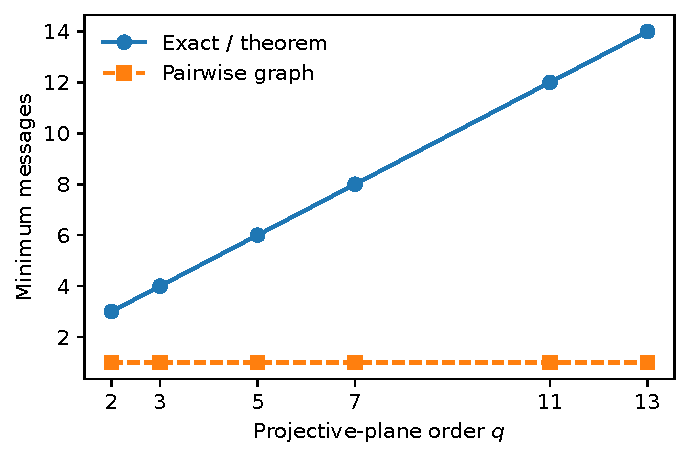
\includegraphics[width=\linewidth]{figures/projective_gap.pdf}
    \vspace{-2ex}
    \centerline{\small (a) Higher-order compatibility gap}
  \end{minipage}\hfill
  \begin{minipage}[t]{0.485\textwidth}
    \centering
    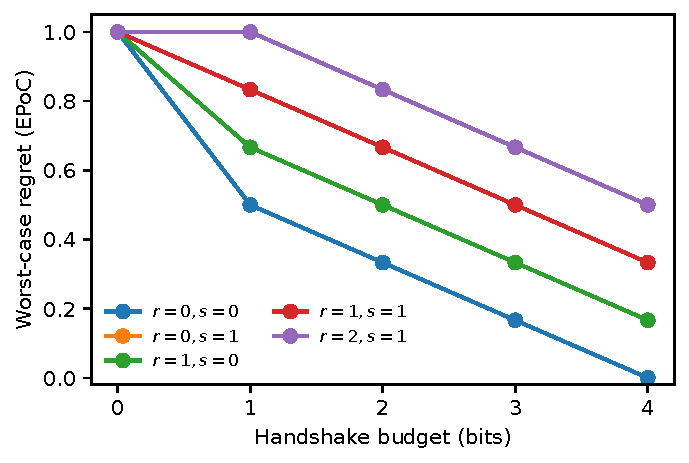
\includegraphics[width=\linewidth]{figures/lever_frontier.pdf}
    \vspace{-2ex}
    \centerline{\small (b) Loss--communication frontiers}
  \end{minipage}
  \caption{\textbf{Exact theoretical predictions.} (a) In projective-plane
  games, the pairwise conflict graph predicts one message while exact MILP and
  Theorem~\ref{thm:projective} require $q+1$. (b) In the 13-lever game,
  communication quantization, sender uncertainty $r$, and hidden dictionary
  uncertainty $s$ add until the physical diameter cap.}
  \label{fig:main}
\end{figure*}

\section{Algorithms and Positive Structure}

\paragraph{Exact finite solver.}
For fixed $M$ and $\epsilon$, introduce binary variables $s_{xma}$ indicating
that sender type $x$ emits message $m$ and takes action $a$, and $r_{ymb}$
indicating receiver response $b$. We solve
\begin{align}
\sum_{m,a}s_{xma}&=1 &&\forall x,\label{eq:sender-simplex}\\
\sum_b r_{ymb}&=1 &&\forall y,m,\label{eq:receiver-simplex}\\
s_{x_\omega ma}+r_{y_\omega mb}&\le1
&&\substack{\forall \omega,m,\ (a,b)\notin\Rset_\omega^\epsilon.}
\label{eq:forbidden}
\end{align}
The formulation has $|X|M|A|+|Y|M|B|$ variables and at most
$|X|+|Y|M+|\Omega|M|A||B|$ constraints.

\begin{proposition}[MILP correctness]\label{prop:milp}
Equations~\eqref{eq:sender-simplex}--\eqref{eq:forbidden} are feasible if and
only if an $M$-message deterministic protocol has regret at most $\epsilon$.
Searching the finite regret levels returns exact $\EPoC(M)$.
\end{proposition}
The proof reads an integral solution as local rules and conversely encodes any
protocol. We independently decode and reevaluate every returned protocol. The
MILP is intended for validation and small design problems, not as a claim of
general polynomial-time tractability.

\paragraph{One receiver and set systems.}
When the sender action is trivial, there is one receiver type, rewards are
binary, and sender type $x$ accepts a set $S_x\subseteq B$, exact coordination
reduces to selecting receiver actions that hit every $S_x$. Thus
$C(0)$ is the transversal number. This specialization connects our framework
to classical one-shot zero-error coordination and set cover
\citep{mceliece1971hide,abroshan2015zero,chvatal1979greedy,feige1998threshold};
we use it for transparent exact and greedy baselines rather than claim the
reduction as new. It immediately implies that exact message minimization is
NP-hard even in this restricted cooperative setting. The standard greedy rule
that repeatedly chooses the receiver action compatible with the most uncovered
sender types returns at most $H_{|X|}$ times the optimal number of messages
\citep{chvatal1979greedy}; classical set-cover lower bounds also transfer
\citep{feige1998threshold}. These are inherited approximation statements, but
they provide a principled baseline for the game-design problem.

\begin{corollary}[Message minimization in set systems]\label{cor:setcover}
Minimum-message exact coordination is NP-hard even with one receiver type, a
trivial sender action, and binary rewards. Greedy returns at most
$H_{|X|}C(0)$ messages in this subclass.
\end{corollary}

The projective construction shows unrestricted set systems require genuinely
higher-order reasoning. Geometric structure restores locality.

\begin{theorem}[Helly rank]\label{thm:helly}
Consider a receiver-only instance with responses in $\mathbb{R}^d$. If every
acceptable response set for a sender/receiver type pair is convex, every
minimal incompatible sender set has size at most $d+1$.
\end{theorem}

\paragraph{Proof.}
If a sender class is incompatible, then for some receiver type the corresponding
convex acceptable sets have empty intersection. Helly's theorem gives a
subfamily of at most $d+1$ with empty intersection. A minimal incompatible set
can be no larger. \hfill$\square$

For intervals ($d=1$), pairwise compatibility is therefore sufficient. With
one receiver type, the minimum messages equal the minimum number of points
stabbing all acceptable intervals, found exactly by repeatedly selecting the
right endpoint of the earliest-ending unhit interval. This contrast precisely
locates a regime in which pairwise graphs are sound.

\paragraph{Sparse epistemic interaction.}
Merge worlds with the same type pair into one acceptable relation and form the
bipartite type-interaction graph on $X\cup Y$. For fixed $M$, assign each sender
variable a pair $(m,a)\in[M]\times A$ and each receiver variable a response
vector in $B^M$. This is a binary CSP on the type graph.

\begin{proposition}[Bounded-treewidth algorithm]\label{prop:treewidth}
Given a width-$w$ tree decomposition, fixed-$M$ threshold feasibility is
solvable in
\[
O\!\left((|X|+|Y|)D^{w+1}\right),\qquad
D=\max\{M|A|,|B|^M\},
\]
up to polynomial local-constraint checks.
\end{proposition}

This dependence is practical for the intended regime of one- to three-bit
handshakes when private-model interactions are sparse.

\section{Metric Action Dictionaries}

Many interoperability problems have a shared physical goal space but private
coordinate systems or action dictionaries. Let $(V,d)$ be a finite metric
space with diameter $D$. The sender observes an estimate $x\in X\subseteq V$;
the true target belongs to a nonempty uncertainty set $U_x\subseteq V$.
Receiver type $g$ is a bijective isometry from local actions $V$ to physical
outcomes $V$. If the receiver chooses local action $b$, the payoff is
$1-d(g(b),t)/D$ for true target $t\in U_x$.

Define the robust assignment cost
\[
\Delta(c,x)=\max_{t\in U_x}d(c,t).
\]

\begin{theorem}[Metric dictionary reduction]\label{thm:metric}
For every $M$,
\[
\EPoC(M)=\frac{1}{D}
\min_{\substack{c_1,\ldots,c_M\in V\\
                   \mu:X\to[M]}}
\max_{x\in X}\Delta(c_{\mu(x)},x).
\]
Thus epistemic protocol design in this family is exactly a robust metric
$M$-center problem. When $U_x=\{x\}$, it is ordinary metric $M$-center and
farthest-first traversal gives a 2-approximation \citep{gonzalez1985clustering}.
\end{theorem}

\paragraph{Proof.}
For message $m$ and receiver isometry $g$, any local response corresponds to a
physical center $c_{g,m}=g(b)$. Because $g$ is bijective, every physical center
is available. The target sets do not depend on $g$, so each receiver type faces
the same minimax center problem for a message class and may implement a common
optimal physical center through $g^{-1}$. Optimizing the message partition and
these centers gives the display. \hfill$\square$

The reduction distinguishes two issues. A private coordinate frame causes no
additional loss once a message identifies a response center; the receiver
inverts its own dictionary. Target uncertainty remains inside $\Delta$ and may
survive full revelation. It also supplies scalable baselines for goal spaces
where exact MILP is unnecessary.

\subsection{Closed form on a noisy cycle}
We now obtain an exact frontier rather than a generic approximation. Let
$K=2h+1$ physical levers lie on a cycle. The sender observes estimate
$x\in\mathbb Z_K$ while the true target satisfies $d_K(x,t)\le r$. Receiver
type $y$ is a nominal frame shift, but the realized local-to-physical
dictionary contains an unobserved bias $\delta$ with $d_K(\delta,0)\le s$.
Local action $b$ selects $b+y+\delta\pmod K$, with payoff
\[
u(t,b,y,\delta)=1-\frac{d_K(b+y+\delta,t)}{h}.
\]
The hidden bias models uncertainty about the process producing the receiver's
action dictionary; neither agent observes it.

An $M$-message protocol quantizes sender estimates into at most $M$ intended
physical centers. The optimal covering radius of an odd $K$-cycle is
\[
\rho_K(M)=\left\lceil\frac{K-M}{2M}\right\rceil.
\]
For an estimate-center distance $d$, sender and receiver uncertainty dilate the
worst physical error to $\min\{h,d+r+s\}$: the triangle inequality gives the
upper bound, and moving target and dictionary in opposite directions attains it.

\begin{theorem}[Additive private-lever frontier]\label{thm:lever}
For $1\le M\le K$,
\[
\boxed{\EPoC_{K,r,s}(M)=
\frac{\min\left\{h,\rho_K(M)+r+s\right\}}{h}.}
\]
Full sender-type revelation leaves the irreducible floor
$\min\{h,r+s\}/h$.
\end{theorem}

The three terms have distinct meanings: $\rho_K(M)$ is communication
quantization, $r$ is target uncertainty seen by the sender, and $s$ is latent
receiver-dictionary uncertainty. The receiver removes its observed nominal
frame by subtracting $y$, but no sender message reveals $t$ or $\delta$.
For tolerance $\epsilon<1$, let
$R=\lfloor\epsilon h\rfloor-r-s$. If $R<0$, no message budget attains the
tolerance; otherwise
\[
C_{K,r,s}(\epsilon)=\left\lceil\frac{K}{2R+1}\right\rceil.
\]
The supplement proves both the cycle covering formula and the exact two-sided
uncertainty dilation.

\section{Unknown Model Channels}

The world set can also encode uncertainty about how private models were
produced. Let a candidate channel $Q$ induce possible worlds $\Omega_Q$ and an
ambiguity family $\mathcal Q$ induce
$\Omega_{\mathcal Q}=\bigcup_{Q\in\mathcal Q}\Omega_Q$. All preceding
results apply to the union instance.

\begin{proposition}[Ambiguity monotonicity]\label{prop:ambiguity}
If $\mathcal Q\subseteq\mathcal Q'$, then
$\EPoC_{\mathcal Q}(M)\le\EPoC_{\mathcal Q'}(M)$ for every $M$, and
$C_{\mathcal Q}(\epsilon)\le C_{\mathcal Q'}(\epsilon)$ for every
$\epsilon$.
\end{proposition}

The statement follows because each protocol is evaluated on a superset of
worlds. Its practical implication is less tautological: a protocol optimized
for one assumed model channel may be maximally fragile even when robust design
substantially reduces the misspecification loss.

The irreducible part has a general cellwise form when the sender's action is
trivial. Let $\Omega(x,y)$ be the latent worlds inducing observed type pair
$(x,y)$ and define
\[
\delta(x,y)=\min_{b\in B}\max_{\omega\in\Omega(x,y)}
 [v_\omega^\star-u_\omega(b)].
\]
\begin{proposition}[Full-revelation floor]\label{prop:full-floor}
In every receiver-only game, if $M\ge |X|$, then
\[
\EPoC(M)=\max_{(x,y):\Omega(x,y)\ne\varnothing}\delta(x,y).
\]
\end{proposition}
The sender can reveal $x$, after which the receiver chooses one robust action
per observed cell $(x,y)$; no sender message can distinguish worlds inside the
same cell. Hence a flat frontier identifies missing observations rather than an
insufficient vocabulary.

For the ambiguous cyclic dictionary, let $K=2h+1$ and let $D_y$ contain the
unobserved additive biases for receiver type $y$. Translation invariance gives
the corollary
\[
\begin{aligned}
\EPoC(K)&=\frac{1}{h}\max_y\operatorname{rad}(D_y),\\
\operatorname{rad}(D)&=\min_c\max_{\delta\in D}d_K(c,\delta).
\end{aligned}
\]
For $D_y=\{0,d_y\}$, this radius is
$\lceil d_K(0,d_y)/2\rceil$. Thus additional sender communication cannot remove
receiver-side uncertainty about its own dictionary.

We instantiate this with an ambiguous cyclic action dictionary. The sender
knows one of 13 physical targets. Receiver type $y\in\{0,1,2,3\}$ specifies a
nominal frame shift, but the true local-to-physical mapping may contain an
additional unobserved bias: respectively $0$, $2$, $4$, or $6$ positions. The
nominal designer assumes zero bias. The robust designer includes both nominal
and biased mappings for each frame. This changes neither agents' observed types
nor the communication budget; it changes only which game model is considered
possible.

\section{Exact Experiments}

All experiments use exact SciPy/HiGHS MILPs or theorem-specific algorithms on a
single CPU; no policy training is performed. The artifact contains raw tables,
29 unit/cross-check tests, deterministic seeds, and scripts for every figure.

\paragraph{Higher-order separation.}
For prime $q\in\{2,3,5,7,11,13\}$, exact projective-plane hitting sets equal
$q+1$ throughout, whereas the empty pairwise graph predicts one message
(Figure~\ref{fig:main}a). At $q=13$, 183 private models require 14 messages.

\paragraph{Additive cyclic uncertainty.}
For $K=13$, two private frames, five $(r,s)$ settings, and zero to four bits,
the general protocol MILP matches Theorem~\ref{thm:lever} on all 25
configurations (Figure~\ref{fig:main}b). An exhaustive audit over every
$r,s\in\{0,\ldots,h\}$ and $M\in[K]$ for $K\in\{3,5,7\}$ adds 169 exact
matches. The $(r,s)=(1,0)$ and $(0,1)$ frontiers coincide; with 13 messages,
regret is $(r+s)/6$, so communication removes quantization but neither hidden
uncertainty source.

\paragraph{Two-dimensional map alignment.}
We use a $5\times5$ physical grid with Manhattan payoff and all eight square
rotations/reflections as private receiver frames. The exact metric-center EPoC
for $M\in\{1,2,4,8,16,25\}$ is
$\{.50,.375,.25,.125,.125,0\}$ (Figure~\ref{fig:secondary}a).
The unrestricted protocol MILP agrees through $M=8$ on two nontrivial frames;
at $M=4$, repeating it with 1, 2, 4, and all 8 frames always returns $.25$.
Farthest-first reaches its worst-case factor two on the audited $3\times3$--
$5\times5$ grids, illustrating both the imported guarantee and the value of
exact protocol design on small maps.

\paragraph{Unknown dictionaries.}
In the asymmetric ambiguity instance (Figure~\ref{fig:secondary}b), a nominally
optimal full-revelation protocol has zero in-model regret but worst-case regret
one over the possible hidden dictionaries. Robust design reduces this to
$1/2$, exactly the cellwise minimax floor. More target detail cannot identify
an unobserved receiver-side model error.

\paragraph{Generic higher-order gaps and intervals.}
Across 140 seeded set systems, the true message requirement is 1.55 times the
pairwise prediction on average and up to three times larger
(Figure~\ref{fig:secondary}c); greedy hitting set averages 1.056 times optimum
and reaches 1.5 on the worst seed. For intervals, right-endpoint greedy matches
the MILP on all 20 audit instances and scales to 10,000 sender types; timing is
a hardware-dependent sanity check, while exactness follows from the theorem.

\begin{table}[t]
\centering
\scriptsize
\setlength{\tabcolsep}{2.0pt}
\begin{tabular}{p{0.42\columnwidth}ccc}
\toprule
Experiment & Baseline & Exact/rob. & Prediction \\
\midrule
Projective plane $q=13$ & 1 & 14 & 14 \\
Random sets, size 10 & 1.00 & 3.00 & -- \\
Cycle $r=s=1$, 4 bits & -- & $1/3$ & $1/3$ \\
$5\times5$ map, $M=4$ & 0.50 & 0.25 & 0.25 \\
Ambiguous dictionary, 4 bits & 1.00 & 0.50 & 0.50 \\
Intervals, audit cases & -- & 20/20 & exact \\
\bottomrule
\end{tabular}
\caption{Representative deterministic results. Baselines are pairwise coloring,
farthest-first, or the best-transferring nominal protocol as appropriate;
random-set entries are means over 20 seeds.}
\label{tab:results}
\end{table}

\begin{figure*}[t]
  \centering
  \begin{minipage}[t]{0.32\textwidth}
    \centering
    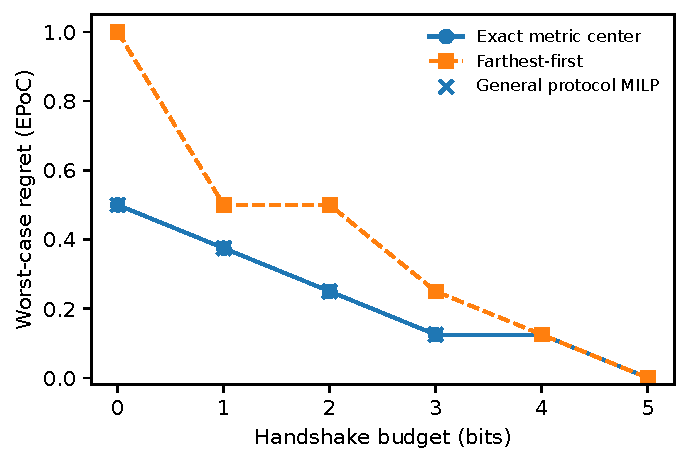
\includegraphics[width=\linewidth]{figures/grid_map_alignment.pdf}
    \vspace{-2ex}
    \centerline{\small (a) Rotated/reflected maps}
  \end{minipage}\hfill
  \begin{minipage}[t]{0.32\textwidth}
    \centering
    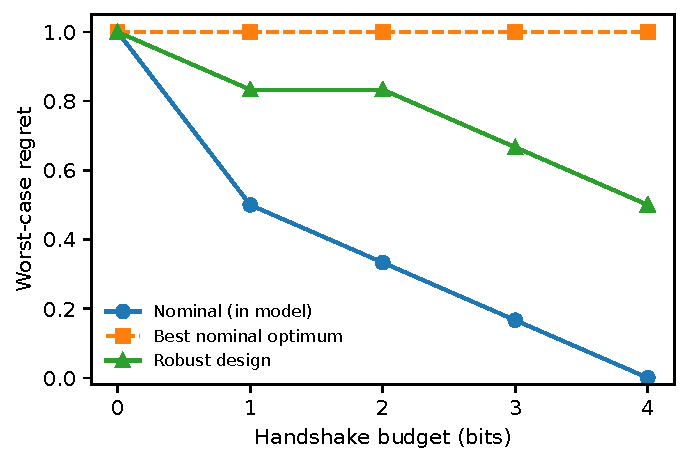
\includegraphics[width=\linewidth]{figures/dictionary_ambiguity.pdf}
    \vspace{-2ex}
    \centerline{\small (b) Model-channel ambiguity}
  \end{minipage}\hfill
  \begin{minipage}[t]{0.32\textwidth}
    \centering
    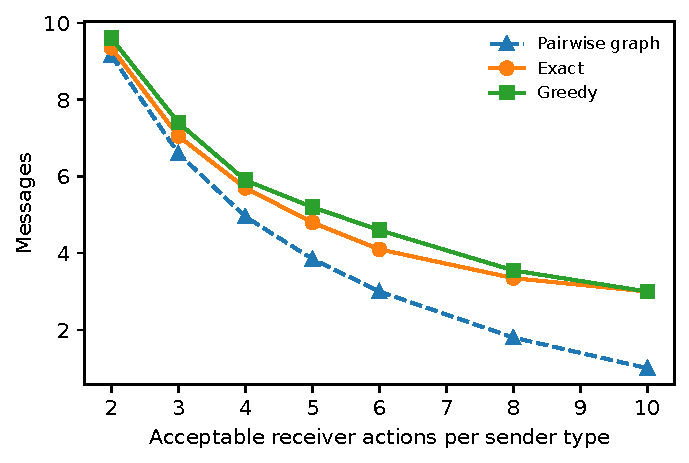
\includegraphics[width=\linewidth]{figures/random_set_systems.pdf}
    \vspace{-2ex}
    \centerline{\small (c) Generic set systems}
  \end{minipage}
  \caption{\textbf{Geometry, robustness, and higher-order structure.}
  (a) The metric reduction matches the general protocol MILP; farthest-first
  can be a factor two worse. (b) Robust design controls an unobserved action
  dictionary but cannot erase its minimax floor. (c) Pairwise coloring
  systematically underestimates higher-order message requirements.}
  \label{fig:secondary}
\end{figure*}

\section{Related Work}

\paragraph{Epistemic game theory and teams.}
Common knowledge formalizes iterated mutual knowledge and has long been central
to coordination and agreement \citep{aumann1976agreeing,geanakoplos1994common}.
Team decision theory studies the joint design of information and decision rules
under decentralized observations \citep{marschak1972teams}, while
communication equilibria study strategic mediation and pre-play reports in
Bayesian games \citep{forges1986communication}. Our agents have identical
payoffs and follow a designed protocol, so incentive compatibility is not the
issue. We instead quantify which private descriptions must be distinguished to
approximate the world-specific team optimum.

\paragraph{Zero-shot coordination and ad hoc teamwork.}
Ad hoc teamwork studies cooperation without prior coordination
\citep{stone2010adhoc,tambe1997flexible}. Other-Play removes arbitrary symmetry
breaking by optimizing cross-play under relabelings \citep{hu2020otherplay};
later methods train diverse partner populations or open-ended cooperative
curricula \citep{strouse2021collaborating,li2023cole}, and recent work targets
cross-environment or evolving-game generalization
\citep{jha2025cross,hui2026efficient}. These methods primarily learn policies.
We instead ask an exact design question: given private game descriptions, what
worst-case value can a bounded interoperability message certify?

Noisy zero-shot coordination is especially close: agents receive noisy private
versions of an underlying Dec-POMDP \citep{anwar2024noisy}. Our finite model
abstracts away training and allows uncertainty about which worlds or
model-generation processes are possible. More importantly, EPoC varies the
message budget and benchmarks against a world-aware oracle, exposing a complete
repairability frontier.

\paragraph{Coordination and zero-error information theory.}
Coordination capacity characterizes distributions implementable with
communication and common randomness \citep{cuff2010coordination,cuff2013distributed}.
Zero-error side-information coding relates exact recovery to graph coloring
\citep{witsenhausen1976zero}; Hide-and-Seek and zero-error coordination study
permissible action sets under private observations
\citep{mceliece1971hide,abroshan2015zero}. Our one-receiver set-system
specialization inherits these classical connections. The distinct emphasis is
payoff-sensitive regret over private \emph{game models}, higher-order
compatibility across strategically interchangeable types, and structural
boundaries linking action cardinality, Helly dimension, and epistemic graph
width. In communication-complexity language, $C(\epsilon)$ is a zero-error
one-way partition complexity for a payoff-threshold relation. Our compatibility
hypergraph makes explicit that the legal cells of this partition can have
higher-order, rather than pairwise, obstructions. The metric-dictionary specialization connects protocol compression to
classical metric clustering and uncertain-center models
\citep{gonzalez1985clustering,xu2025uncertain}. We use the farthest-first
guarantee of \citet{gonzalez1985clustering}; the new modeling step identifies
when that geometric objective is exactly the oracle-relative coordination
loss.

\paragraph{Decentralized control.}
General decentralized partially observed control is computationally hard
\citep{bernstein2002complexity}. Rather than approximate a general Dec-POMDP,
we isolate a one-shot interoperability layer and characterize exactly when its
complexity collapses to 2-SAT, interval stabbing, or bounded-treewidth CSP.

\section{Implications for Multi-Agent Design}

\paragraph{Handshake symbols should encode strategic classes.}
A natural engineering approach is to hash, cluster, or serialize private model
parameters. Theorem~\ref{thm:hypergraph} gives a different target: a message
class is valid only when all of its models admit a common continuation for each
receiver type. Consequently, representational similarity is neither necessary
nor sufficient. Two numerically different models can share a symbol when their
acceptable action relations align, while pairwise-compatible models may still
fail collectively.

\paragraph{Minimal incompatibilities are diagnostic certificates.}
A hyperedge identifies a smallest collection of local models that cannot share
a handshake symbol. Such certificates can be returned alongside an infeasible
MILP to explain why a protocol vocabulary is too small. Theorem~\ref{thm:helly}
shows when diagnosis is local: in $d$-dimensional convex response spaces, at
most $d+1$ models witness failure. The projective family shows that no universal
pairwise certificate exists without structural assumptions.

\paragraph{A flat frontier calls for sensing, not more language.}
The additive-cycle, map, and ambiguous-dictionary experiments distinguish loss caused by
compressed conventions from loss caused by absent information. Once
$\EPoC(M)$ reaches its floor, increasing the message alphabet cannot help; the
system must improve sensing, model calibration, message direction, or the
information revealed to the other agent. Thus the frontier is also a design
diagnostic for deciding whether to allocate resources to communication or to
better private models.

\section{Limitations and Conclusion}

The present theory is deliberately narrow. It treats two agents, deterministic
one-way pre-play messages, finite worst-case world sets, and predominantly
synthetic games. Positive-regret randomization, interactive protocols, learned
or continuous private models, many-agent coalitions, and Bayesian objectives
can change both the operational interpretation and the complexity. Our exact
MILP is a validation tool rather than a large-scale solver, and classical
hitting-set hardness still applies to an important subclass.

Within this scope, the results give a precise answer to a basic interoperability
question. The cost of private game models is a payoff-sensitive staircase, not
a binary property. Its communication threshold is governed by higher-order
compatibility, which pairwise diagnostics can underestimate without bound; yet
convexity, intervals, and sparse type interactions restore tractability. The
closed-form lever family further separates mismatch that a handshake repairs
from uncertainty that no message can remove. These distinctions provide a
compact theoretical foundation for designing and auditing communication among
heterogeneous cooperative agents.

\bibliography{references}

\end{document}
